\documentclass{article}
\usepackage{amsmath}
\usepackage{ragged2e}
\usepackage{bookmark}
\usepackage{wrapfig}
\usepackage{hyperref}
\usepackage{textgreek}
\usepackage{caption}
\usepackage{graphicx}
\usepackage[top=2cm]{geometry}
\title{\textbf{Mushroom Classification using C4.5 Algorithm}}
\author{$
Anjali^{[\hyperref[author:anjali]{1}]}, 
Sreevallabh^{[\hyperref[author:sreevallabh]{2}]}, 
Bhanu Prakash^{[\hyperref[author:bhanu]{3}]}, 
Abhinav^{[\hyperref[author:abhinav]{4}]}, 
Pranesh^{[\hyperref[author:pranesh]{5}]}$}
\date{\today}
\begin{document}
\maketitle

\section{Abstract}
This paper focuses on using the C4.5 algorithm to classify different species of mushrooms according to important morphological characteristics. The collection includes a variety of mushroom samples, each distinguished by characteristics including habitat, color, odour, and cap form. A decision tree model is constructed using the C4.5 method, with a focus on feature selection and information gain to improve model accuracy.

The project involves data preprocessing, splitting into training and testing sets, and training the C4.5 decision tree model. The resulting model is evaluated against the testing set using standard classification metrics, including accuracy, precision, recall, and F1 score.

This technique has practical implications for everyday uses and scientific research, such as helping foragers differentiate between edible and dangerous mushrooms. The study offers a data-driven method for identification purposes and sheds light on the efficiency of the C4.5 algorithm for classifying mushrooms. The results offer useful insights for anyone interested in practical uses of mushroom classification as well as machine learning practitioners.

\vspace{.25cm}
\setlength{\leftskip}{-.5cm}
\textbf{Key Words:} Mushroom Classification $\cdot$ C4.5 $\cdot$ Decision Tree $\cdot$ Information Gain $\cdot$ Data pre-processing

\section{Contents}\label{sec:contents}

The following is the structure of the paper.
\begin{enumerate}
    \item \hyperref[sec:intro]{Introduction}
    \item \hyperref[sec:dc]{Data Cleaning}
    \item \hyperref[sec:eda]{Exploratory Data Analysis}
    \item \hyperref[sec:transfromation]{Data Transformation}
    \item \hyperref[sec:building]{Model Building}
    \item \hyperref[sec:eval]{Model Evaluation}
    \item \hyperref[sec:conclusion]{Conclusion}
    \item \hyperref[sec:references]{References}
\end{enumerate}

\section{Introduction}\label{sec:intro}
The mushroom dataset consists of different mushrooms intended for classification applications. Each mushroom is described by a number of features, like its physical properties and much more. Each item includes a number of rows and columns with information on various aspects, including `color', `odor', and `cap-shape'. This massive dataset is a useful tool for estimating trends and creating machine learning models that can tell the difference between deadly and edible mushrooms.

The complete dataset has around 8100 rows of data and each row contains 23 features describing individual mushroom according to their attributes.

\textbf{Features:} class $\cdot$ cap-shape $\cdot$ cap-surface $\cdot$ cap-color $\cdot$ bruises $\cdot$ odor $\cdot$ gill-attachment $\cdot$ gill-spacing $\cdot$ gill-size $\cdot$ gill-color $\cdot$ stalk-shape $\cdot$ stalk-root $\cdot$ stalk-surface-above-ring $\cdot$ stalk-surface-below-ring $\cdot$ stalk-color-above-ring $\cdot$ stalk-color-below-ring $\cdot$ veil-type $\cdot$ veil-color $\cdot$ ring-number $\cdot$ ring-type $\cdot$ spore-print-color $\cdot$ population $\cdot$ habitat

All the columns are discrete and are ordinal data type. When processing these columns, they are converted into factor type for further analysis of the data set.


\section{Data Cleaning}\label{sec:dc}
Initial analysis of the dataset had been performed and it was found out that there are no missing elements and no null values. So we can say that the dataset provided is very clean. There are no duplicate rows in the dataset.

In the initial analysis we found out that the feature stalk-root has `\textit{?}' in its unique values. From further analyzing this feature, it is found out that 2480 rows have `\textit{?}' as its value. This shows that there is a requirement for further analysis of the individual features.

\section{Exploratory Data Analysis}\label{sec:eda}
As we have found out that there is a requirement of analyzing every feature of the dataset, we first calculate the number of unique values in the dataset. Using the number of unique values, we can remove the features with very high or very low cardinality. The following is the analysis of different features:


\begin{wrapfigure}{r}{0.35\textwidth}
    \begin{minipage}{\linewidth}
        \raggedleft
        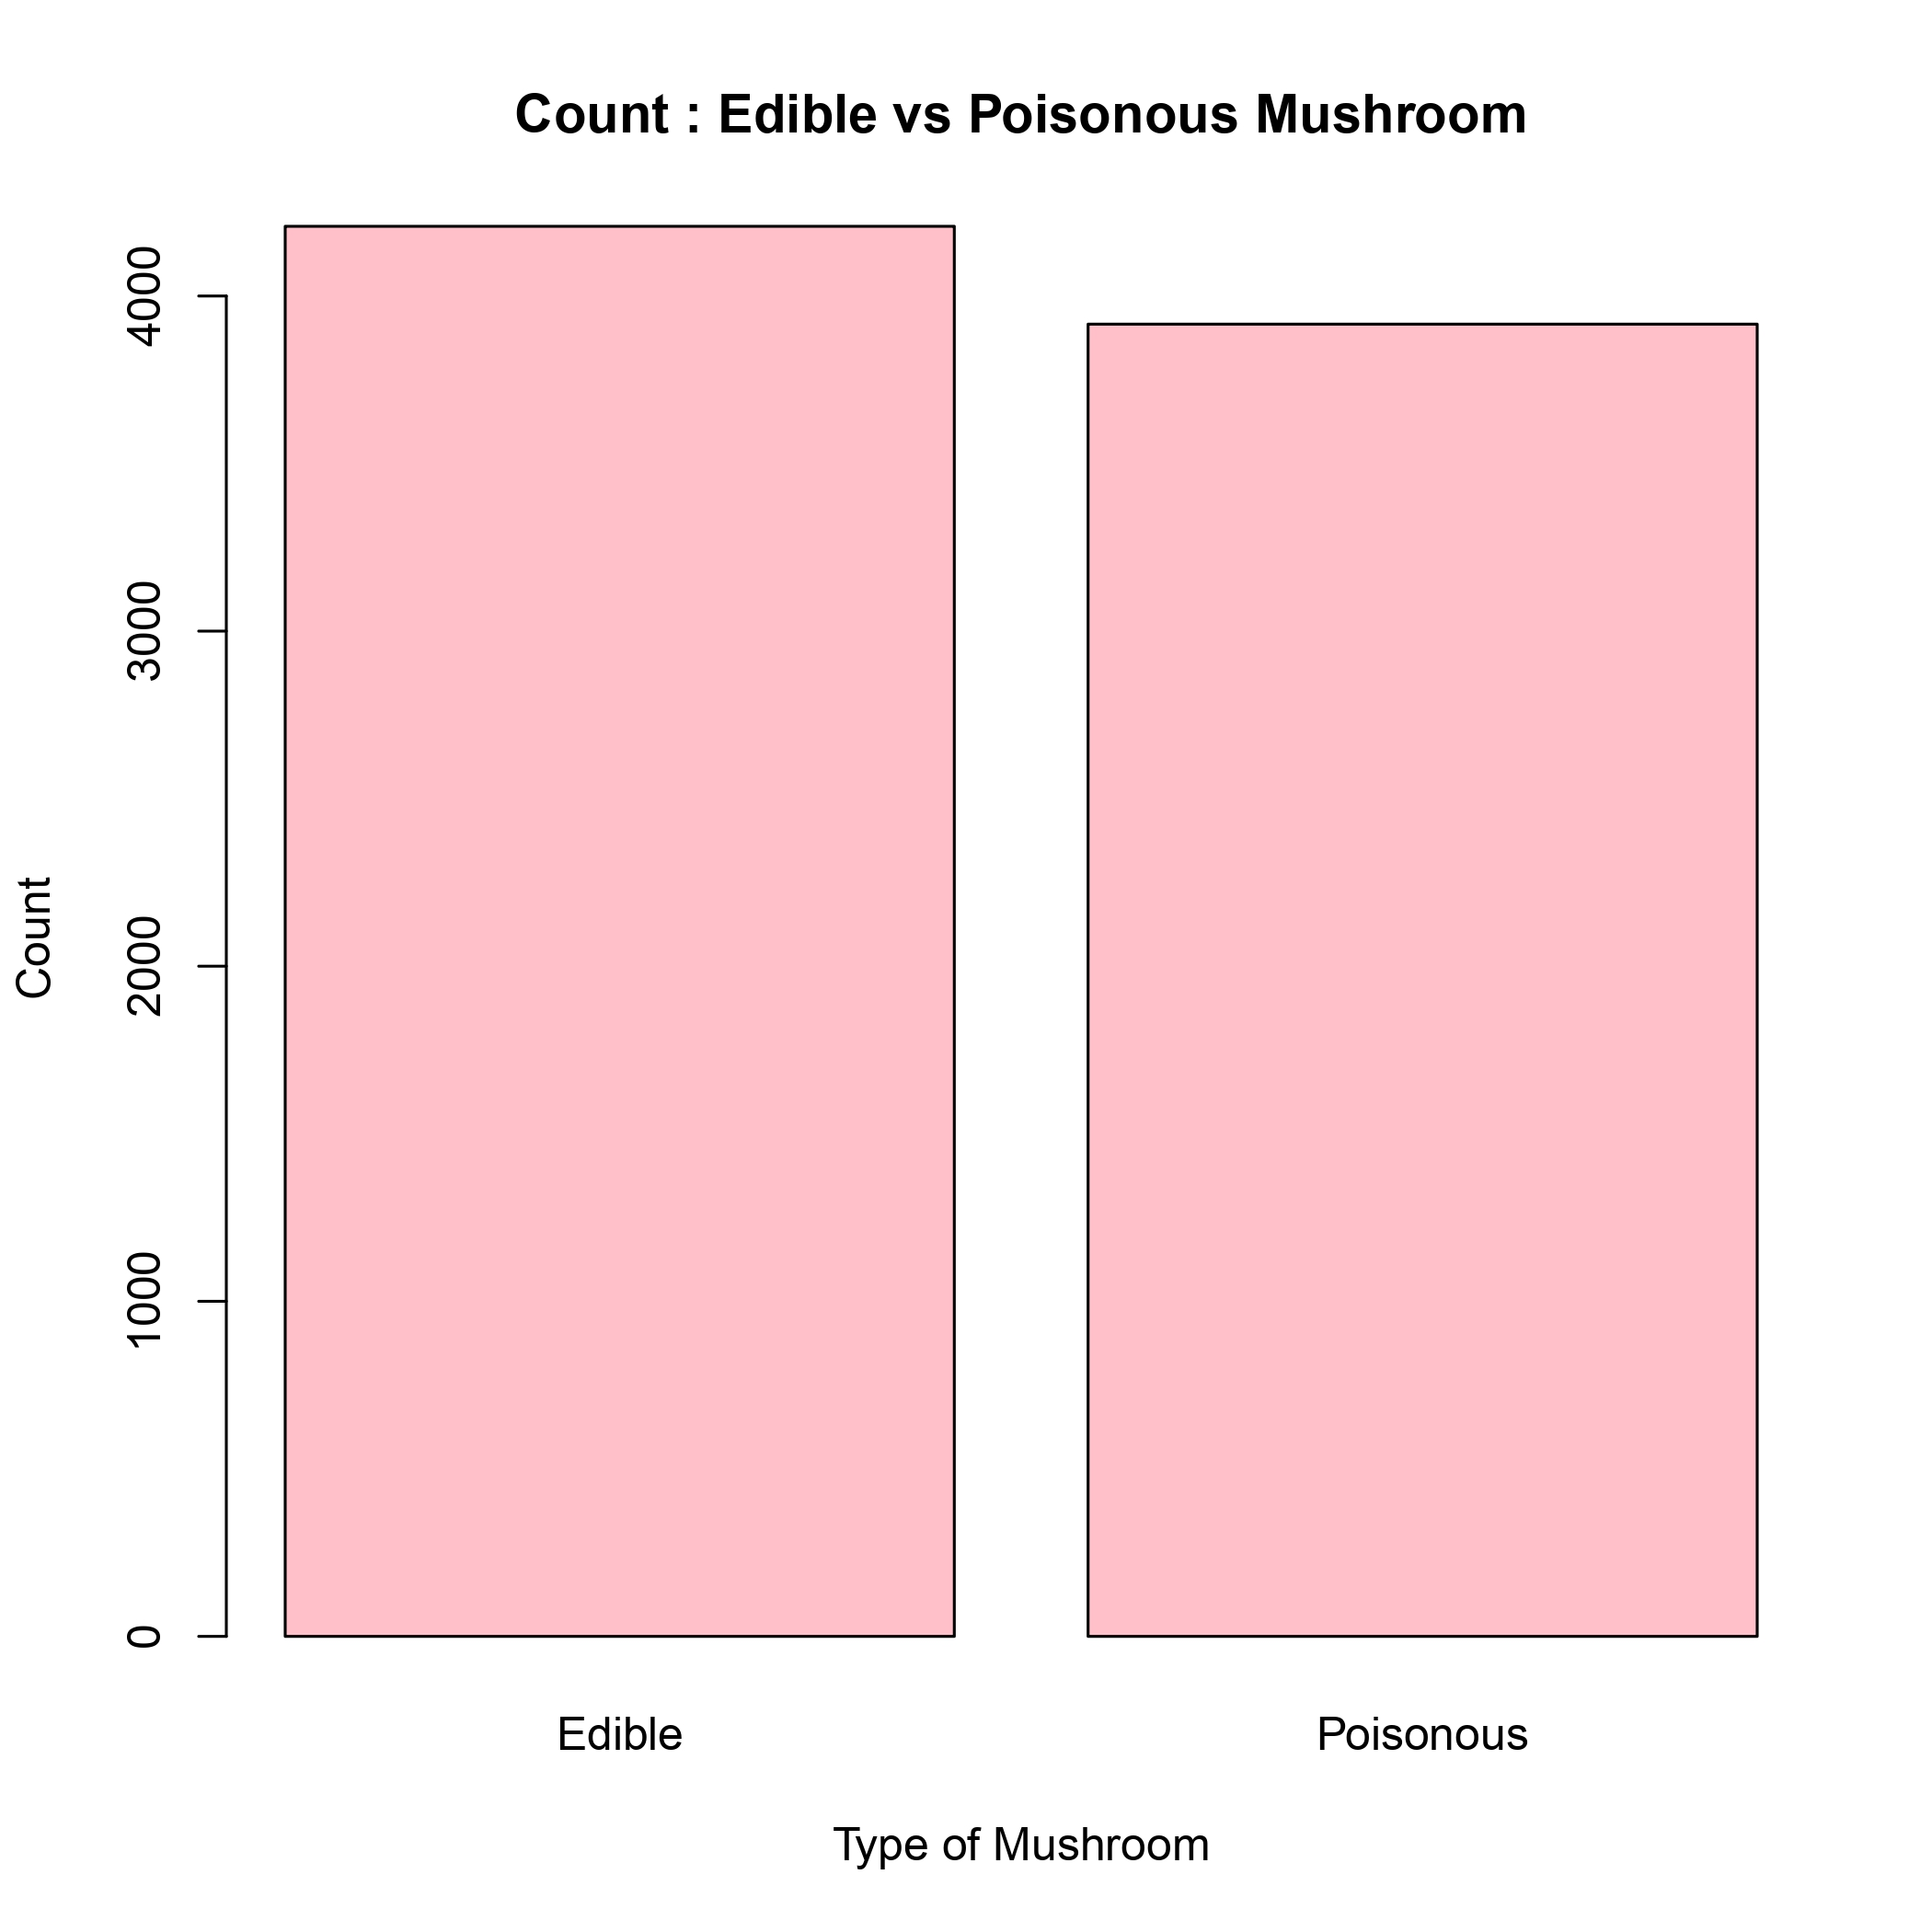
\includegraphics[width=0.9\linewidth]{./images/Rplots_pages-to-jpg-0001.jpg}
        \captionsetup{width=0.7\linewidth}
        \caption{Frequency of unique values in `class'}
        \label{img:1}
    \end{minipage}
\end{wrapfigure}


In \hyperref[img:1]{Figure 1}, we are analyzing the feature `class' which is our target variable. It has 2 unique values \textit{e} and \textit{p} \textit{i.e.,} edible  and poisonous. Around 52\% of mushrooms are edible. As we can see that the frequency of positive and negative data labels are almost equal, we can conclude that we can use a classifier as model for this data set. We can also conclude that the dataset is balanced.

\subsection{Data Modeling}\label{subsection:dm}
From \hyperref[img:2]{Figure 2}, we analyze the gill features of the mushrooms: `gill-attachment', `gill-spacing', `gill-size', `gill-color' and `gill-shape'. Out of the above mentioned features, `gill-attachment' have a very low cardinality of 2. Due to very low cardinality these features are not helpful in classifying the data.

\vspace{.25cm}
\begin{figure}[ht]
    \centering
    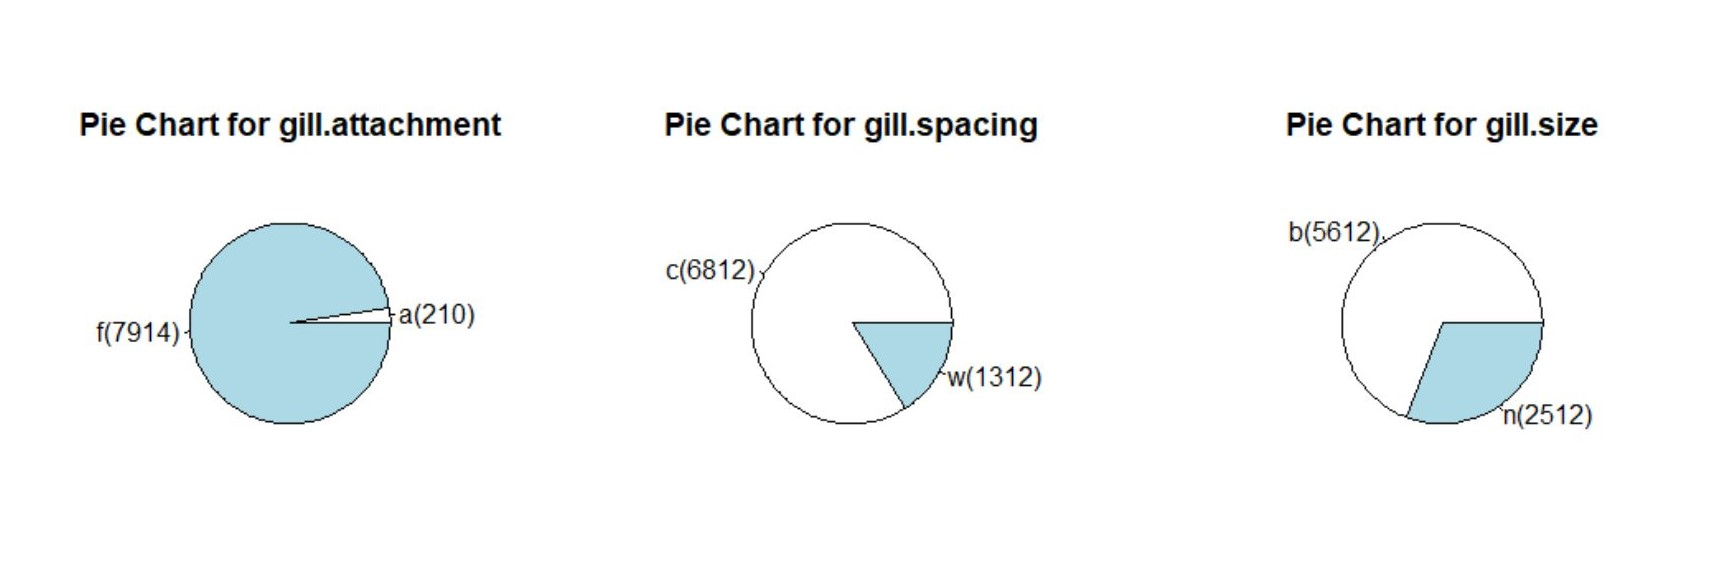
\includegraphics[width=0.8\textwidth]{./images/Gill.jpg}
    \caption{Frequency of unique terms in `gill-attachment', `gill-spacing', `gill-size'}
    \label{img:2}
\end{figure}

A cardinality threshold of less than or equal to 2 was employed in the study. Specifically, the attributes `bruises' and `stalk-shape' exhibit merely two distinct values each, as we can see in \hyperref[img:3]{Figure 3}. Conversely, the attribute `veil-type' is characterized by a singular unique value. This analysis provides a nuanced perspective on the diversity and distribution of unique values within the dataset. Due to large number of features having variable cardinalities, $Principal Component Analysis^{[\hyperref[subsection:pca]{1}]}$ is required for selecting the best features to train the model.


\begin{figure}[ht]
    \centering
    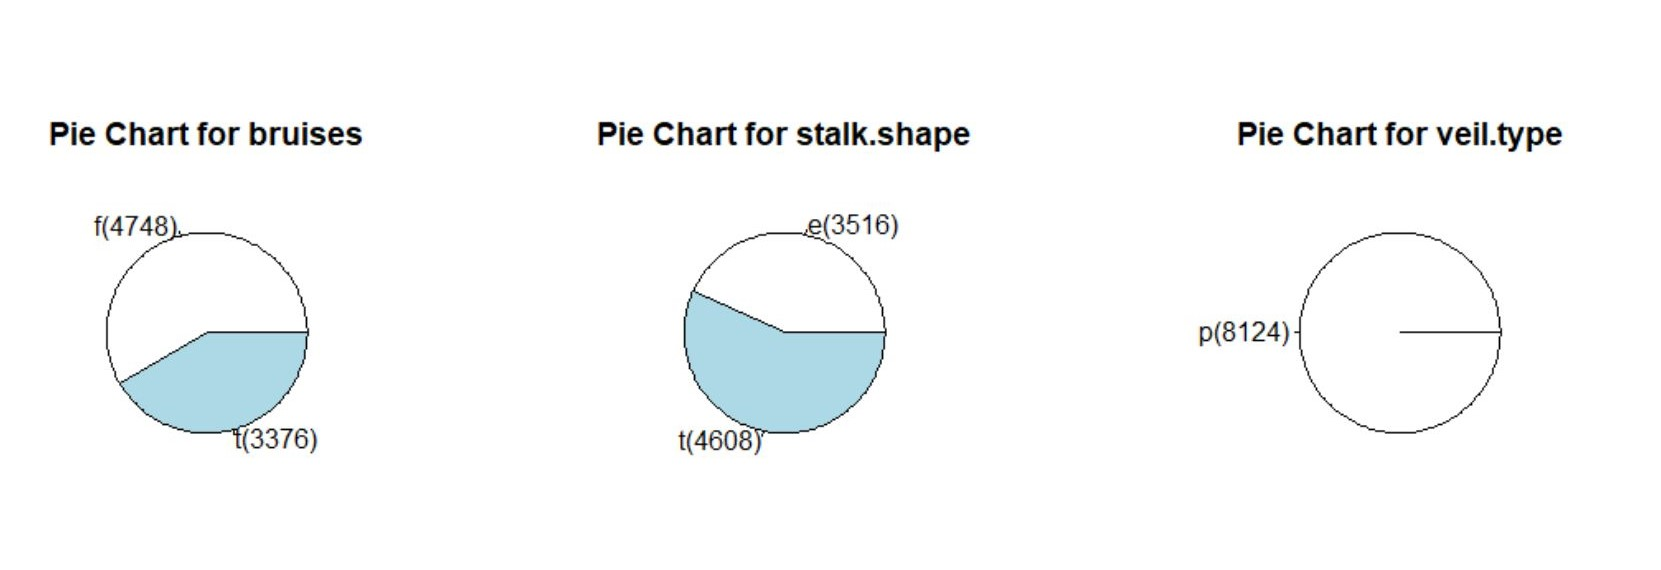
\includegraphics[width=0.8\textwidth]{./images/bruises_veil-type_stalk-shape.jpg}
    \caption{Frequency of unique terms in `bruises', `stalk-shape', `veil-type'}
    \label{img:3}
\end{figure}

\textbf{Removed features} (after Data Modeling): bruises $\cdot$ gill-attachment $\cdot$ gill-spacing $\cdot$ gill-size $\cdot$ stalk-shape $\cdot$ veil-type. Now we have a dataset of \textbf{17} features for further analysis.


\subsection{Principal Component Analysis}\label{subsection:pca}
\begin{wrapfigure}{l}{0.6\textwidth}
    \begin{minipage}{\linewidth}
        \centering
        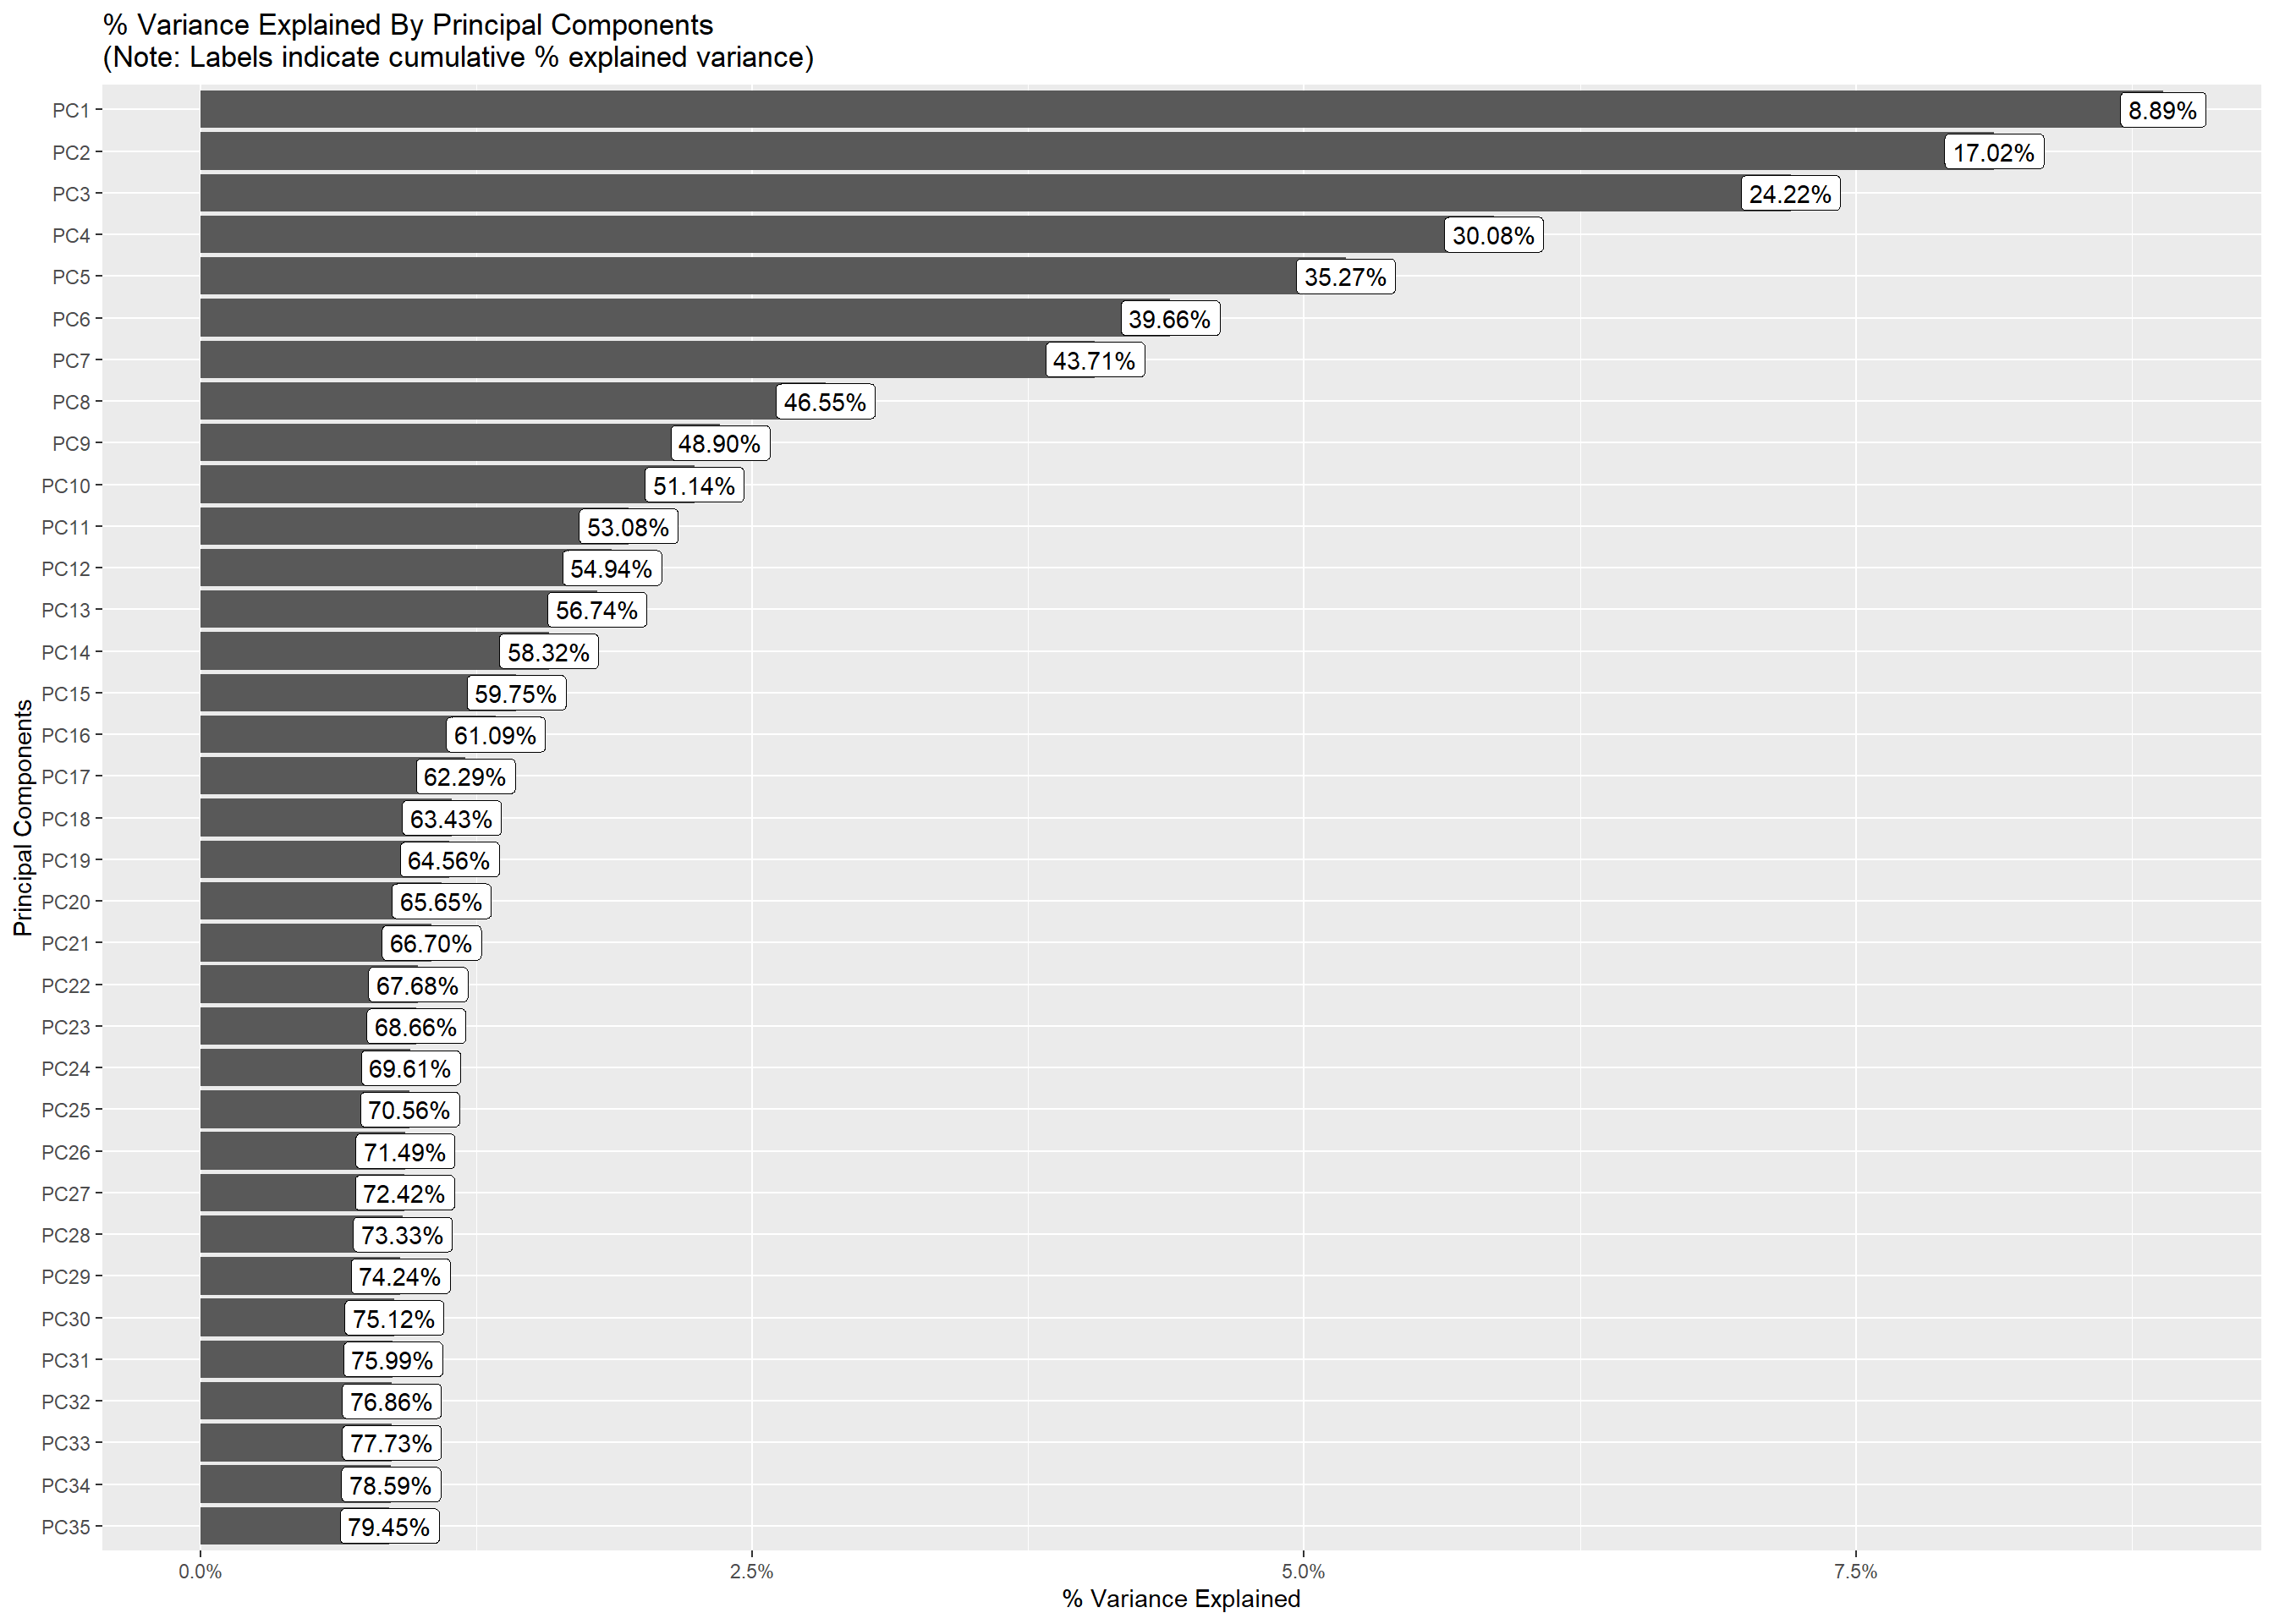
\includegraphics[width=0.9\linewidth]{./images/principal_component_analysis-1.png}
        \captionsetup{width=0.8\linewidth}
        \caption{Frequency of unique values in `class'}
        \label{img:4}
    \end{minipage}
\end{wrapfigure}

Due to variable cardinalities in the features of the data, we need to perform Principal Component Analysis. We can extract the features with maximum variance. Here we have maximized the variance of the features and extracted the top 35 features from all the unique features from the data set. This plot is against the main feature label `class' \textit{i.e.,} the unique values `e' (edible) and `p' (poisonous).

As we can see in \hyperref[img:4]{Figure 4}, some of the main features are extracted from PCA that are required for building the model include `odor' and `spore-print-color'. As we have extracted some important features using PCA, to understand the relationship between the features, we perform the `Correlation Analysis' to get the best related features to our target feature \textit{i.e.,} `class'.

\subsection{Correlation Analysis}\label{subsection:corr}
In the context of data preparation for the decision tree model, attention was focused on understanding correlation patterns among attributes. Attributes showing low correlation with the target variable underwent a deliberation process for potential removal, with the goal of model streamlining while maintaining the accuracy of the model.

\begin{figure}[ht]
    \centering
    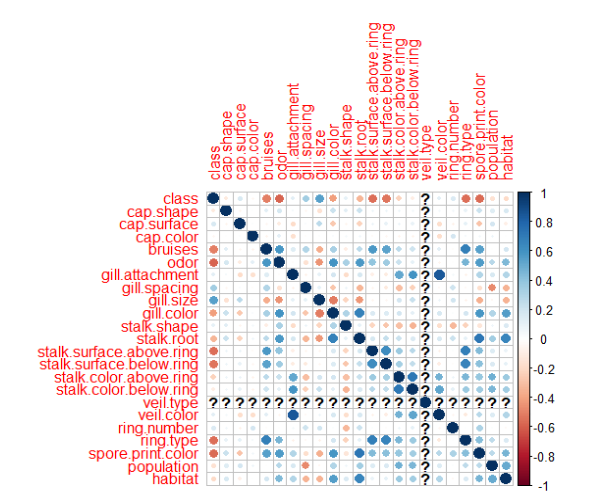
\includegraphics[width=0.8\textwidth]{./images/Correlation_Plot.png}
    \caption{Correlation Analysis}
    \label{img:5}
\end{figure}

In \hyperref[img:5]{Figure 5}, we have performed correlation analysis for all the features because we have to assure that there is no feature that has a high correlation value with the target class has not been removed in the previous steps of preprocessing.

\textbf{Assumption}

\begin{equation}
    \rho \geq 0.5 
\end{equation}

The incorporation of a correlation threshold played a crucial role in this context, aiding in the identification and exclusion of attributes exhibiting weak correlations. Additionally, the exploration of high correlations between attributes led to considerations about managing multi co-linearity. Finally, after considering the threshold($\rho$) values the features got reduced to bruises $\cdot$ odor $\cdot$ gill-size $\cdot$ stalk-surface-above-ring $\cdot$ stalk-surface-below-ring $\cdot$ ring-type $\cdot$ spore-print-color when matched against the target feature `class'.

\section{Data Transformation}\label{sec:transfromation}
During the data transformation stage, we utilized the \texttt{as.factor()} function to convert each attribute. This important step was to properly managing categorical data within the dataset. The \texttt{as.factor()} function played a vital role in giving a numeric identity to categorical variables, ensuring they align well with subsequent analyses. This technical move allowed for a smooth integration of categorical information into a numeric framework, creating a solid foundation for statistical and machine learning procedures.

\section{Model Building}\label{sec:building}
\subsection{Data Splitting}
We split the dataset random in the ratio of $2:1$ for training and testing purposes respectively. We have also set the seed to \textbf{123} for reproducibility when run even in a difference setting.

\subsection{The C4.5 Algorithm}
Decision Tree Classifier is a type of machine learning technique, that makes decisions by splitting the data into subsets based on the values of input features. It's like a flowchart where each node represents a decision based on a specific feature, and each branch represents a possible outcome. The goal is to create a tree that helps make predictions or decisions.

C4.5 is an algorithm used to build decision trees. Its main job is to decide on which features to split and when to stop splitting. It works by finding the feature that provides the best split, \textit{i.e.,} it separates the data into subsets that are more homogeneous in terms of the target outcome. The algorithm repeats this process recursively for each subset until a stopping condition is met, creating a tree structure.

Here is the working of the \textbf{C4.5 Algorithm}.
\subsubsection{Attribute Selection}
The algorithm recursively selects the attributes which have the least entropy until there is only one attribute being 100\% of the class.

\subsubsection{Entropy Calculation}
It measures the impurity or disorder inside of the data.
\begin{equation}
    Info(D) = - (\sum_{i=1}^{m}p_i log_2(p_i))
\end{equation}
Here, $p_i$ is the $i^{th}$ feature from the attribute set. The attribute with the least entropy gets the highest priority to be present in the decision tree.

\subsubsection{Calculation of Information Gain}
It is the measure of the information retrieved from an attribute to form the total information received.

\begin{equation}
    Info_A(D) = \sum_{j=1}^{\nu} \frac{|D_j|}{|D|}*(H(D_j))
\end{equation}

\begin{equation}
    Gain(A) = Info(D) - Info_A(D)
\end{equation}

Here we have the Information gain for the given attribute. Now we have find the gain ratio for setting up the classifier.

\subsubsection{Split Info}
Measures the amount of data separation caused by the feature.
\begin{equation}
    SplitInfo_A(D) = -\sum_{j=1}^{\nu} \frac{|D_j|}{|D|}*log_2(\frac{|D_j|}{|D|})
\end{equation}

\subsubsection{Gain Ratio}
Adjusting the Information Gain to account for the potential bias towards the features with many values.


\begin{equation}
    GainRatio(A) = \frac{Gain(A)}{SplitInfo_A(D)}
\end{equation}

\subsubsection{Recursive Tree Building}
Based on the best feature at that instance from the $GainRatio$ function, we split the data and add the feature that is split into the current tree node. Now this node acts as a root element for the next recursive step of the algorithm.

\subsubsection{Stopping Conditions:}
\begin{itemize}
    \item If all instances in a node belong to the same class, or if all attributes have been used for splitting, further partitioning is unnecessary. In such cases, the node becomes a leaf node, and the class label is assigned accordingly.
    \item If the number of instances in a node falls below a specified threshold, further splitting may lead to over fitting. Setting a minimum number of instances for a node helps control the tree's complexity.
    \item The algorithm evaluates the information gain for potential splits. If the calculated information gain is below a certain threshold, the split might not contribute significantly to the overall classification accuracy. Thus, the splitting is stopped.
    \item To prevent the tree from becoming overly deep and overly specific to the training data, a maximum depth is often imposed. If a node reaches this depth during the tree-building process, it becomes a leaf node.
\end{itemize}

\section{Model Evaluation}\label{sec:eval}

\subsection{Model Prediction}
We try to classify the test data using decision tree from test samples, which we have split from the total data set while building the model. For model prediction, we need to convert feature value to the same format as in the training data. If feature value is not present in the tree, then we return the majority class.

\subsection{Evaluation Metrics}
Using confusion matrix, we measure the performance of the model in terms of \textit{accuracy}, \textit{precision}, \textit{F1-Score} and \textit{ROC Curve}.

\subsubsection{Confusion Matrix}
\centering
\begin{tabular}{|c|c|c|}
    \hline
    \multicolumn{1}{|c|}{} & +ve & -ve \\
    \hline
    +ve & 1 & 2 \\
    \hline
    -ve & 1293 & 1415 \\
    \hline
\end{tabular}

\raggedright
\vspace{.25cm}
From the above confusion matrix we have found out the following values:
\begin{itemize}
    \item \textit{Accuracy}: 52.25\%
    \item \textit{Precision}: 52.25\%
    \item \textit{Recall}: 100\%
    \item \textit{F1-Score}: 68.63\%
\end{itemize}

\begin{figure}[ht]
    \centering
    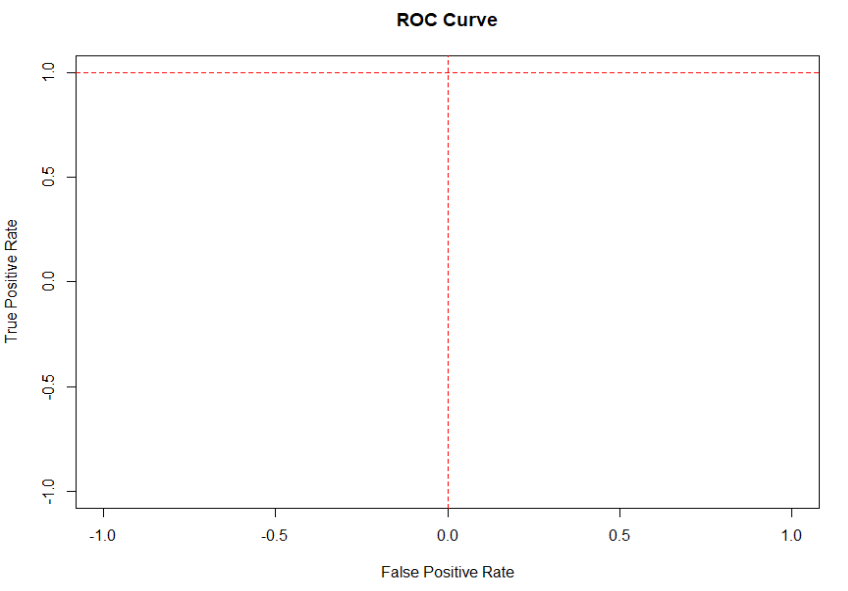
\includegraphics[width=0.8\textwidth]{./images/ROC Curve.png}
    \caption{ROC Curve}
    \label{img:6}
\end{figure}

\begin{justify}
\subsection{\textit{k}-fold Cross Validation}
\textit{k}-fold Cross Validation is a technique used to assess the performance of a machine learning model, such as the one employed in mushroom classification. The process involves dividing the dataset into `\textit{k}' equally sized folds or subsets. 

The model is then trained and evaluated `\textit{k}' times, with each fold serving as the test set once and the remaining folds as the training set. This method helps ensure that the model's performance is robust and not influenced by a specific data split. 

Here, \textit{k}-fold Cross Validation allows us to gauge how well the model generalizes to different subsets of the dataset. By iteratively training and testing on various partitions, we obtain a more reliable estimate of the model's effectiveness in distinguishing between edible and poisonous mushrooms. 

The average performance metrics across all folds, such as accuracy, precision, recall, and F1-score, provide a comprehensive evaluation of the model's overall capability. This approach aids in identifying potential issues like over fitting or under fitting, contributing to a more trustworthy and dependable mushroom classification model.


\subsection{Modes for Improvement}
As we have seen that the `accuracy' and `precision' for the test data set is very low. We converted our data entries which are of ordinal data into factors. This leads to loss of information, sensitivity to levels. It's important to weigh these disadvantages against the benefits and consider them in the context of the specific machine learning algorithm and dataset characteristics.

Here are some of the methods in which we can improve the efficiency of the algorithm:

\subsubsection{Data Pruning}
When a decision tree is built, many of the branches will reflect anomalies in the training data due to noise or outliers. Tree pruning methods address the problem of over fitting the data by decreasing the complexity and making the tree easy to comprehend. They are usually `faster' and more efficient in classifying independent test data.

We have not used $Data Pruning$ in out model because after performing the correlation analysis, six features were remaining. If we have performed tree pruning, further information would have been lost. 

\subsubsection{Using Alternate Algorithms}
Better and enhanced versions of `C4.5 Algorithm' like `CART' (Classification and Regression Trees) can be used for classifying this dataset. `CART' uses $GiniIndex$ as its measure for classification. The $GiniIndex$ is calculated as:

\begin{equation}
    Gini(D) = 1 - \sum_{i=1}^{m}p_i^2
\end{equation}
\begin{equation}\label{equation:1}
    Gini_A(D) = \frac{|D_1|}{|D|}Gini(D_1) + \frac{|D_2|}{|D|}Gini(D_2)
\end{equation}
\begin{equation}
    GiniIndex(A) = \Delta Gini(A) = Gini(D) - Gini_A(D)
\end{equation}

From \hyperref[equation:1]{equation 8}, we can see that the $GiniIndex$ naturally lends itself to binary splits, making it well-suited for decision trees that create binary splits at each node.

\subsubsection{Feature Engeneering}
Feature engineering aids the C4.5 algorithm by transforming raw data into a more representative and predictive format. Techniques such as one-hot encoding and binning refine categorical variables, while scaling ensures numerical features contribute uniformly. This refinement process empowers C4.5 to better classify from the data, manifesting robust and efficient classification outcomes.

\section{Conclusion}\label{sec:conclusion}
Focused on mushroom classification, this research centers on leveraging the C4.5 algorithm to categorize distinct mushroom species based on vital morphological traits. The application of the C4.5 decision tree model prioritizes feature selection and information gain, resulting in heightened model accuracy. Navigating through crucial stages like data preprocessing, partitioning into training and testing sets, and model training, the project culminates in evaluating the model against the testing set. This assessment employs standard classification metrics, including accuracy, precision, recall, and F1 score, validating the model's efficiency.

As a result, we have got ~55\% efficiency after testing the test sample split from the dataset in the ratio of $2:1$ and after performing \textit{k}-fold Cross Validation. The current implementation meets the basic requirements, but there are areas that could be improved. 

\section{References}\label{sec:references}

\subsection{Authors}\label{authors}
\setlength{\leftskip}{.2cm}
All the authors belong to Indian Institute of Information Technology, Sri City. 

\setlength{\leftskip}{-.3cm}
\textbf{Batch:} UG-3.

\setlength{\leftskip}{-.3cm}
\textbf{Group No.} 15

\vspace{.5cm}
\setlength{\leftskip}{-.5cm}
\textbf{Team Member Details}

\begin{enumerate}
    \item \label{author:anjali} \textbf{Anjali Kumari:} \href{mailto:anjali.k21@iiits.in}{\underline{anjali.k21@iiits.in}}, S20210010021.
    \item \label{author:sreevallabh} \textbf{Sreevallabh Karanam:} \href{mailto:sreevallabh.k21@iiits.in}{\underline{sreevallabh.k21@iiits.in}}, S20210010110.
    \item \label{author:bhanu} \textbf{Bhanu Prakash Bhaskarla:} \href{mailto:bhanuprakash.b21@iiits.in}{\underline{bhanuprakash.b21@iiits.in}}, S20210010041.
    \item \label{author:pranesh} \textbf{Pranesh S:} \href{mailto:pranesh.s21@iiits.in}{\underline{pranesh.s21@iiits.in}}, S20210010181.
    \item \label{author:abhinav} \textbf{Abhinav Mars:} \href{mailto:abhinav.t21@iiits.in}{\underline{abhinav.t21@iiits.in}}, S20210010229.
\end{enumerate}

\setlength{\leftskip}{-.5cm}
\textbf{Contributions}

\begin{enumerate}
    \item \label{author:anjali} \textbf{Anjali Kumari:} Data preprocessing and Exploratory Data Analysis.
    \item \label{author:sreevallabh} \textbf{Sreevallabh Karanam:} Model Building, Model Training, Performance Analysis.
    \item \label{author:bhanu} \textbf{Bhanu Prakash Bhaskarla:} Model Building, Model Training, Performance Analysis.
    \item \label{author:pranesh} \textbf{Pranesh S:} Data Transformation and Feature Scaling.
    \item \label{author:abhinav} \textbf{Abhinav Mars:} \textit{k}-fold Cross Validation and Further Improvements.
\end{enumerate}

\subsection{Bibliography}\label{bibliography}

\begin{enumerate}
    \item \href{https://github.com/Anjali19991/Mushroom-Classification}{Project Code: Github}
    \item \href{https://hanj.cs.illinois.edu/bk3/bk3_slidesindex.htm}{Data Mining Concepts and Techniques} By Jiawei Han, Micheline Kamber, Jian Pei
\end{enumerate}

\end{justify}
\end{document}